\documentclass{standalone}
\usepackage{tikz}
\usetikzlibrary{calc}

\begin{document}
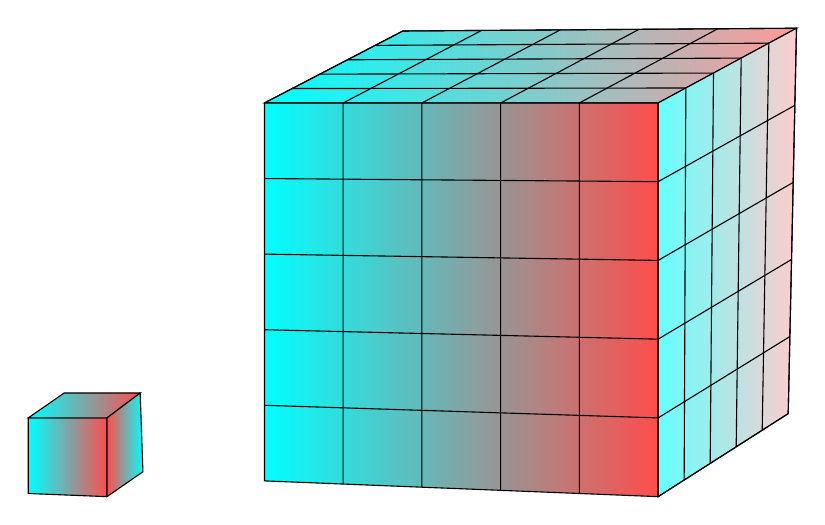
\begin{tikzpicture}

\coordinate (Center) at (0,0);
\coordinate (a) at (0,0.2);
\coordinate (b) at (0,5);
\coordinate (c) at (5,0);
\coordinate (d) at (5,5);
\coordinate[yshift=30,xshift=50] (a1) at (a);
\coordinate[yshift=26,xshift=50] (b1) at (b);
\coordinate[yshift=30,xshift=47] (c1) at (c);
\coordinate[yshift=27,xshift=50] (d1) at (d);

\coordinate (A) at (-3,0.04);
\coordinate (B) at (-3,1);
\coordinate (D) at (-2,1);
\coordinate (C) at (-2,0);
\coordinate[yshift=10,xshift=13] (A1) at (A);
\coordinate[yshift=9,xshift=13] (B1) at (B);
\coordinate[yshift=9,xshift=12] (D1) at (D);
\coordinate[yshift=9,xshift=13] (C1) at (C);



\shade[draw,left color=cyan, right color=red!70] (a) -- (b) -- (d) -- (c) -- cycle;
\shade[draw,left color=cyan, right color=red!40] (b) -- (b1) -- (d1) -- (d) -- cycle;
\shade[draw,left color=cyan!60, right color=red!20] (d) -- (d1) -- (c1) -- (c) -- cycle;

\draw (b) -- (b1) -- (d1) -- (c1) -- (c) -- (d) -- (b);

\foreach \x in {0.2,0.4,0.6,0.8}
\draw ($(a)!\x!(c)$) -- ($(b)!\x!(d)$) -- ($(b1)!\x!(d1)$);
\foreach \x in {0.2,0.4,0.6,0.8}
\draw ($(a)!\x!(b)$) -- ($(c)!\x!(d)$) -- ($(c1)!\x!(d1)$); 
\foreach \x in {0.2,0.4,0.6,0.8}
\draw ($(b)!\x!(b1)$) -- ($(d)!\x!(d1)$) -- ($(c)!\x!(c1)$);   

%\draw[step=1cm,gray] (-10,-10) grid (10,10);


\shade[draw,left color=cyan, right color=red!70] (A) -- (B) -- (D) -- (C) -- cycle;
\shade[draw,left color=cyan, right color=red!70] (B) -- (B1) -- (D1) -- (D) -- cycle;
\shade[draw,right color=cyan, left color=red!70] (D) -- (D1) -- (C1) -- (C) -- cycle;


%\draw (Center) circle (2pt);
%\node[below] at (a) {a};
%\node[below] at (b) {b};
%\node[below] at (c) {c};
%\node[below] at (d) {d};
%\draw[color=red] (a1) circle (2pt) node[below] {a1};
%\draw[color=red] (b1) circle (2pt) node[below] {b1};
%\draw[color=red] (c1) circle (2pt) node[below] {c1};
%\draw[color=red] (d1) circle (2pt) node[below] {d1};

\end{tikzpicture}

\end{document}